\section{ICML Reviewer comments}

\subsection*{Reviewer ZW8t}

\subsubsection*{Weaknesses}

\begin{itemize}
    \item Clarity of variable definitions in the proposed framework needs to be addressed. In Equation (1), the explanation of variables is confusing. For example, it is unclear what $\mathbf{o}_t$ represents. Are these observations outputs of prior sub-agent calls? Why use the subscript $t$?
    \item The notion of ``prior sub-agent calls'' (lines 112--113) is unclear. What distinguishes $\mathbf{o}_t$ from $\mathbf{s}_t$? What exactly do sub-agent calls return?
    \item The distinction between $\mathbf{s}_t$ and $\mathbf{z}_t$ (lines 119--120) is unclear.
    \item In Figure 2, there is no visible arrow from the agent state to the LLM, despite the text suggesting that the LLM accepts the agent state as input.
    \item Figure and section organization could be improved; figures are sometimes isolated at the ends of pages.
    \item Line 114 defines $\mathbf{a}_t$, but Section 3.2.2 uses both $\mathbf{a}_t$ and $\mathbf{y}_t$ as conditions.
    \item The loss $\mathcal{L}_1$ is described as optimizing the agent projector, but its formulation appears to optimize $\mathbf{y}_t$, creating inconsistency.
    \item Similar ambiguity exists for $\mathcal{L}_2$; the role of the loss function is unclear.
    \item The right panel of Figure 2 is difficult to interpret. It is unclear how $\hat{\mathbf{z}}_t$ is derived, whether it is predicted solely by the LLM, and what the projection from $\mathbf{s}_t$ to $\mathbf{z}_t$ represents conceptually.
    \item Figure 5 refers to blue text annotations that are not present.
    \item Section 4.4 scenarios are difficult to understand without consulting the appendix.
    \item The source of natural language explanations used in Stage 2 training is not described.
    \item Chess-specific metrics such as G-eval and Diff in Table 1 are not explained.
    \item Insufficient details are provided about baselines, including how supervised task experts are trained and how GPT-4o uses agents via tool calling.
    \item No ablation study isolates the effects of Stage 1 versus Stage 2 training.
    \item Section 4.6 mentions LoRA but provides no details or comparisons.
    \item It is unclear what constitutes training versus evaluation data when claiming generalization in Section 4 and Table 1.
    \item Related contemporary work on latent chain-of-thought reasoning is omitted.
    \item Broken hyperlinks and presentation issues reduce readability.
    \item Figure 1 appears too early and contains domain-specific terminology not yet introduced.
    \item Figure 1 contains unlabeled bar plots whose meaning is unclear.
\end{itemize}

\subsubsection*{Questions}

\begin{itemize}
    \item Is there an ablation comparing the use of $\mathbf{s}_t$ versus $\mathbf{z}_t$? What does $\mathbf{z}_t$ contribute beyond using $\mathbf{s}_t$ directly?
    \item What exactly is a ``verbalized action''? Is it generated by the sub-agent, and how does it differ from normal language tokens?
    \item In Figure 1, why does policy-without-search performance drop when pretraining data increases to 30M tokens? What do the bars represent?
    \item In Section 4.3, how often does LLAMIA demonstrate nuanced understanding in practice? Is there any human evaluation or quantitative analysis?
    \item In Figure 5, LLAMIA outputs appear verbose. How should verbosity be interpreted in terms of output quality?
\end{itemize}


\subsection*{Reviewer LEvg}

\subsubsection*{Weaknesses}

\begin{itemize}
    \item The paper lacks formal rigor in its decision-theoretic framing. Claims relating LLM generation to MDPs, POMDPs, and hierarchical RL are made without precise definitions.
    \item Claims of long-horizon planning are not convincingly supported, relying primarily on chess comparisons with GPT-4o.
    \item Comparing a heavily fine-tuned specialized model with general-purpose LLMs using few-shot prompting is not a fair comparison.
    \item Insufficient explanation is provided for the generalization experiments on vision and persuasion tasks, which are relegated to the appendix.
    \item It is unclear how these generalization tasks relate to planning and reasoning, which is the core motivation of the paper.
    \item Presentation issues include unexplained color coding in Table 1 and undefined terms such as ``SOTA (SFT)''.
    \item Figures are poorly placed, with multiple consecutive figures at the end of the paper while key experimental details are deferred to the appendix.
\end{itemize}

\subsection*{Questions}

\begin{itemize}
    \item What do the different color boxes in Table 1 represent?
    \item What methods are referred to by ``SOTA SFT'' in Table 1?
\end{itemize}


\subsection*{Reviewer HUaR}

\subsubsection*{Weaknesses}

\begin{itemize}
    \item The mathematical formalization introduces unnecessary complexity and symbol overloading, leading to inconsistencies in notation and conditioning.
    \item The POMDP framing is misleading since the optimization objectives would require reinforcement learning, which is not used.
    \item The conditioning in the loss formulation appears contradictory, as the model is conditioned on tokens it is also tasked with predicting.
    \item Related work connecting policy networks with LLMs in robotics and autonomous driving is not discussed or differentiated.
    \item Integration with traditional search algorithms is unclear, and the ``Internal Search'' mechanism lacks detail and ablation analysis.
    \item The role of the $\langle \text{InvokeAgent} \rangle$ token is unclear and not demonstrated in examples or datasets.
    \item The experiments focus heavily on chess, limiting claims of general-purpose planning.
    \item Experiments on vision and persuasion tasks lack sufficient methodological detail.
    \item The limitations section is narrow and lacks discussion of broader impacts, particularly given the persuasion experiments.
\end{itemize}

\subsubsection*{Questions}

\begin{itemize}
    \item How does GPT-4o use Lc0 as a tool in practice?
\end{itemize}

% This document was modified from the file originally made available by
% Pat Langley and Andrea Danyluk for ICML-2K. This version was created
% by Iain Murray in 2018, and modified by Alexandre Bouchard in
% 2019 and 2021 and by Csaba Szepesvari, Gang Niu and Sivan Sabato in 2022.
% Modified again in 2023 and 2024 by Sivan Sabato and Jonathan Scarlett.
% Previous contributors include Dan Roy, Lise Getoor and Tobias
% Scheffer, which was slightly modified from the 2010 version by
% Thorsten Joachims & Johannes Fuernkranz, slightly modified from the
% 2009 version by Kiri Wagstaff and Sam Roweis's 2008 version, which is
% slightly modified from Prasad Tadepalli's 2007 version which is a
% lightly changed version of the previous year's version by Andrew
% Moore, which was in turn edited from those of Kristian Kersting and
% Codrina Lauth. Alex Smola contributed to the algorithmic style files.
\begin{comment}
    \section{Feedback}
Continous vs Discrete

\begin{enumerate}
    \item What defines a foundational model?
    \begin{enumerate}
        \item (Bommasani et al. 2021). Foundation models constitute large-scale AI models that are pre-trained on vast amounts of general data and that can be adapted for downstream applications (e.g., by fine-tuning them through further training on application-specific data). Through this pre-train and adapt approach they expedite the development of innovative AI products and services and accelerate the accessibility of high-performance AI solutions in various industries (Teubner et al. 2023).
        \item With scaling, foundation models are becoming increasingly good at performing tasks they were not explicitly trained for, thereby broadening the scope of applications achievable by a single model without the need for additional training data or fine-tuning (Brown et al. 2020).When needed, task-specific performance can be further enhanced through fine-tuning or effective prompt engineering techniques; (Liu et al. 2023; Niu et al. 2020).
        \item Following Bommasani et al. (2021, p. 1), we define a foundation model as ``any model that is trained on broad data that can be adapted to a wide range of downstream tasks''. Through this combination of task-agnostic pre-training and subsequent fine-tuning, foundation models enable new approaches to building and deploying AI systems.
        \item Emergent Capabilities The first key feature of foundation models is the emergence of behavioral capabilities that were not explicitly constructed, nor expected, by human developers, which frequently is referred to as in-context learning (Min et al. 2022)
        \item \cite{XXXFlava} a true foundation model in the vision and language space should not only be good at vision, or language, or vision-and language problems–it should be good at all three, at the same time.
    \end{enumerate}
    \item What would characterize a foundational decision model
    \item What constitutes an FDM
    \item Why Chess
    \somesh{P2 @Harini ChessFormer, AlphaZero}
    \begin{itemize}
        \item 
    \end{itemize}
    \item Emergent Properties across Large Decision Models
    \item Why search or runtime compute
    \item Why Language and Decisions
    
\end{enumerate}








Planning is a key task in real-world scenarios whiuch has not been solved in the generality needed by any foundation models [cite: Yann Le Cun tweeted a reference for this]. 

Foundation models for decision making should look like... creation of adapters - one per environment. We provide one approach - RLQA to create foundation models for decision making.

Task specific specialist models have their own disadvantages such as limited generalizability. To get the best of these two approaches, researchers have proposed coupling LLMs with specialist policies using toolformers, agentic models etc. [cite: ].



However, this loose coupling cannot solve tasks which require the LLM to understand the specialist policy. Some concrete examples of such tasks include commentary generation in games, language conditioned policy adaptation, language based behavior generalization etc. To bridge this gap, we propose an approach called RLQA, where we tightly couple the LLM and the specialist policy using a policy-language adapter. In this paper, we present an approach to train this adapter, provide benchmarks to test the efficacy of the coupled LLM and specialist policy and provide demonstrations of tasks where our RLQA approach significantly outperforms other popular approaches in literature either in terms of accuracy or efficiency. In this paper, we restrict attention to chess, but our approach is extensible to any planning problem in general.

Fig-1 with descriptive caption - inference pipeline
One paragraph on approach and motivation, novel tasks, datasets and benchmarks


Generalist agent for a single environment - can generate/simulate multiple behaviors in a text controlled manner. A method to align an agent and an LLM a foundation model in decision making and decision understanding
Emergent properties on unseen tasks
Bridging the gap between specialized agents and LLMs via our own connectors:
1. to solve greater tasks which cannot be solved by these independently or weakly coupled
2. example commentary generation, fine-tuned behavior cloning, conditional decision making - example opponent/environment conditioning


Contributions need to be differentiated - Benchmark vs Algorithm vs Model \somesh{1 Algorithm, 3 Datasets, 4 Benchmarks How should we do this?}

Benchmark: Are we providing an arena for testing other RL agents? \somesh{Yes}


Effectiveness of Generalized Decision Making - needs to be defined... \somesh{Conditional Decision Making - Similar to Behavior, Explanation - Directly state annotation, game analysis. Agent identification- Cheating Detection, Improving search - LLMCTS :P}

\begin{enumerate}
    \item What is a foundational model ? A foundation model is any
model that is trained on broad data (generally using self-supervision at scale) that can be adapted (e.g., fine-tuned) to a wide range of downstream tasks; current examples include BERT [Devlin et al.2019], GPT-3 [Brown et al. 2020], and CLIP [Radford et al. 2021]
\end{enumerate}

\somesh{What to capture: What does a foundational decision making model need, an LLM and a policy or representation learning model, and a generalized method to connect these. What should it be trained on? Large Unsupervised number of decisions, and rewards/evaluation.}
\subsection{Contribution}
1. Foundation Decision models
    1.1 Behaviour cloning in few shots, or IFT with 10\% of the data, one model vs finetunes.  Table 1
    1.2 Behaviour stylometry: Unseen task, Comparable or better results with, 15\% of  shots across 20,40,112,High Ranked, GMs, Bots, Elo identification, Time formats table 1.3 
2. We are able to get the strongest known raw policy 
https://arxiv.org/pdf/2402.04494

2. Comparison against Llama3.1 405B with tool calling to Lc0 + MCTS, and GPT-4o with Evaluation and next best moves from Lc0 + MCTS. (All tables) Projection tokens in FDM perform better than tool calling on more than 30x larger LLMs. (All tables)

3. What can an FDM do? Results breakdown why are FDMs needed
    1. Only LLM tasks: position description
    2. Only Engine tasks: puzzle
    4. One model to all
    3. Neither finetune nor agentic task: commentary, position difficulty, rating,
Breadth of tasks with the star-graph

4. What data goes into an FDM:
    1. Self-supervised large scale data (Existing positions and their evals)
    2. Demonstrations from humans (BC)
    3. Complex Instruction data (small scale, downstream applications)

5. Results and analysis
Appendix Lucena

6. Extend this to other envs.


OPenreview
1. Towards building a foundation decision model



4. Commentary generation, 

5. Decision Understanding
https://aclanthology.org/P18-1154.pdf
https://aclanthology.org/P19-1597.pdf
https://arxiv.org/pdf/2212.08195
5. Emergent Abilities unlocked via jointly training with agent projections: Breadth of tasks
6. Towards fdm ?

1. Using Decisions or Policy as a modality unlocks downstream capabilities. (LLaVA sense - DT is an input as opposed to a competition)
    Relevant Results:
        a. State Value Multi Choice, Annotation, Commentary, BOT classification, Puzzles Understanding, Game Masking
        b. Downstream capabilities such as game or
state commentary generation, we outperform SOTA models and even upto 10x larger LLMs
assisted with super-human engines

2. LLMs with Optimal Policy are effecient 0-shot behavior cloners (simulators)
    a. Behavior cloning all results

3. LLMs are strong and efficient look ahead models
    3.1 LLMs themselves model N-step lookahead better than agent trained on that task (Performance, Data required)
    3.2 LLMs that learn look ahead modelling improve downstream performance (tasks)

4. 
\section{Learning to Look Ahead}
Any problem that requires planning can be described by

\begin{enumerate}
    \item A problem statement or current state (S)
    \item A proposed solution or Action (A)
    \item Approximate feedback (F)
    \item An agent or policy (P) that can generate sub-optimal or near-optimal actions.
\end{enumerate}
Current research solves this task by using (P) obtained from self-supervised learning on large amounts of data, as a heuristic to do a "search", or a chain of intermediate actions, which progressively lead to $max(F)$. The resulting search, the tree of actions, is able to solve the problem statement better.

In this work we try to answer the following questions

\begin{enumerate}
    \item Can LLMs exploit an agent's heuristic to plan N-step ahead? We know that Lc0's NN has a policy of only 2600, + MCTS 3500
    \somesh{Note to self: For general problems the LLM itself is the agent}
    \begin{enumerate}
        \item We further train the agent to predict the optimal actions -> +21
        \item We train RLQA to predict the optimal actions -> +53
        \item We train RLQA to predict the optimal actions and the chain-of-thought (the best path in the tree of actions) to it -> +143
    \end{enumerate}

    \item What is the value of the explicit search (
\end{enumerate}
1. Can LLMs exploit an agent's heuristic to plan N-step ahead?
    1.1. We train an agent to predict the optimal policy -> +21
    1.2. We train Agent+LLM to predict the optimal policy -> +53
    1.3. (Train-time) We train Agent+LLM to predict the ToT + optimal policy -> +143 -> Input: FEN(Board) -> Output: Evaluation and next best moves until 30 depth (3500 Elo)
    1.4. (Train-time) We train Agent+LLM to predict the ToT + optimal policy -> +143 -> 
        Input: FEN(Board)
        Output: Evaluation + (next best moves + environment verbalization) until 30 depth (3500 Elo)
        Ablations 1. Only ground truth 2. Synthetic w Ground truth (Agadmator vs Crowd sourced vs Random Tokens)
    1.5. (Train-time) We train Agent+LLM to predict the ToT + optimal policy -> +143 -> 
        Input: FEN(Board)
        Output: Evaluation + (next best moves + annotation/commentary) until 30 depth (3500 Elo)
    1.6. (Train-time) We train Agent+LLM to predict the ToT + optimal policy -> +143 -> 
        Input: FEN(Board)
        Output: Evaluation + (next best moves) until 30 depth (3500 Elo) + Commentary/Annotation of the 3500 Elo
    1.7. (Game-level commentary) We train Agent+LLM to predict the ToT + optimal policy -> +143 -> 
        Input: FEN(Board)
        Output: Evaluation + (next best moves) until 30 depth (3500 Elo) + Commentary of the 3500 Elo
    
2. What is the value of the explicit search tokens?
    2.1. We train an agent to predict the (ToT + optimal policy), Infer w/o ToT -> +76

3. How can we train an LLM to plan with progressive Tree of thoughts
    3.1 We IFT the optimal path and pruning -> +36
    3.2 We IFT the optimal path and pruning progressively -> +75
        Input -> FEN
        Output -> Eval + Next-best move

O1 analogy, 


Parameter Count Trend
1. Concluding that what may not work for smaller models may not translate to stronger models

\section{Model}
\emph{Getting representations from an expert engine, adapting it and then feeding the adapted representation to an LLM to do the following downstream tasks - multi-choice chess annotation, checkmate puzzles, state-value multi-choice, encoding <--> PGN (verbalization) bidrectional; need to check if adding the encoding helps at all, \textbf{behavior simulation (ACM 2018, Maia Chess) - one model, multiple Elos (and also one specific player), accuracy, commentary generation (beating SOTA based on state-level commentary generation - we will do trajectory-level)}}

We consider the standard MDP based RL framework with the usual notation. Let $\pi^*$ denote a learnt (optimal) policy using any RL based approach that also yields $Q^*$, the optimal state-action values. We then look at the following problems:
\begin{enumerate}
    \item Policy Explanation: Given $\pi^*$, $Q^*$, the corresponding state space $\mathcal{S}$ and a state featurizer (could be a textual featurizer), we create a dataset $\widehat{\mathcal{D}}$ of $\{(S_t, f_t, A_t, Q_t,)_{t=0}^T \}_{i \in \mathcal{D}}$, where:
    \begin{enumerate}
        \item $i$ represent an episode from $\mathcal{D}$ which is an offline (can be batch or online as well) dataset of episodes/trajectories.
        \item $t \in \{0, T\}$ represents the step in the episode.
        \item $S_t \in \mathcal{S}$ represents the state at time $t$.
        \item $f_t$ represents the verbalized features of $S_t$.
        \item $A_t \sim \pi^*(S_t)$ represents the action chosen at time $t$ using policy $\pi^*$.
        \item $Q_t = Q^*(S_t, A_t)$ represents the action-value starting from state $S_t$ and choosing action $A_t$.
    \end{enumerate}
    Using this dataset, $\widehat{\mathcal{D}}$, as a first task, we finetune an LLM to predict the $Q$ values given the rest of the sequence. For the purpose of this experiment, we consider the following potential list of environments:
    \label{ref:Candidate envs for text}
    \begin{enumerate}
        \item \url{https://github.com/carla-simulator/carla}
        \item \url{https://github.com/microsoft/TextWorld}
        \item \url{https://github.com/ronentk/TextLabs}
        \item \url{https://github.com/IBM/visual-hints-textworld-rl}
        \item \url{https://github.com/google-deepmind/open_spiel}
        \item \url{https://github.com/Farama-Foundation/Minigrid}
        \item \url{https://github.com/allenai/ScienceWorld}
        \item \url{https://github.com/fidler-lab/social-driving}
        \item \url{https://github.com/google-deepmind/android_env}
        \item \url{https://github.com/facebookresearch/nocturne}
        \item \url{https://github.com/microsoft/CyberBattleSim}
    \end{enumerate}
\end{enumerate}

10M games existing
600B positions pre-existing SF-16

No. of possible positons >>> 600B positions pre-existing SF-16

Twitter:

Dataset: -> Low time
Agent -> Time series
Training -> Low time
Evaluations -> Transsuasion time



\section{Extension}
\subsection{Video Planning}
For long videos LLMs are used to generate video plans, \cite{VideoStudio,DirectorGPT} we will generate multi scene ads, we will plan it with FDM .

1. Optimal Decision making -> Ad Plan Generation from title, intent
2. Conditional Decision making -> Ad Plan generation given scene, conditions etc.
3. GDU/Commentary: Explain a scene (describe, 

1. Decision Making -> Video Plan Generation (memorable, likes/views)
2. Generalised Decision Making (Scene Fill / Complete) -> Behaviour Cloning (GDM)
3. -> Decision Understanding
\subsection{MultiGame DT}

\newpage
SFT: Transsuasion [Vicuna(13B)]: 0.31
Agent: Chronos-base (univariate): 0.09
Agent: Chronos-base (self+industry): 0.17
Pretrain: LLAMIA[Vicuna(13B) + Chronos-base (self+industry)]: 0.28
Pretrain+SFT: LLAMIA[Vicuna(13B) + Chronos-base (self+industry)]: 0.49

\somesh{Qualitative analysis of what LLM learnt from TS agent}
\somesh{Add LLM hidden state into chronos embedding}
LLM Learnt Optimal Policy:



LLAM:
    Input:
        Board position embedding + FEN 

    Output:
        (+7.2) Moves: m1 m2 m3 m4
        Also PV1: 6.1 m1, m2, m3


Finetuned Vicuna:
    Input:
        Board FEN, SV, Evaluation is (+7.2) on move m1

    Output: 
        m2 m3 m4
\begin{figure}[!h]
    \centering
    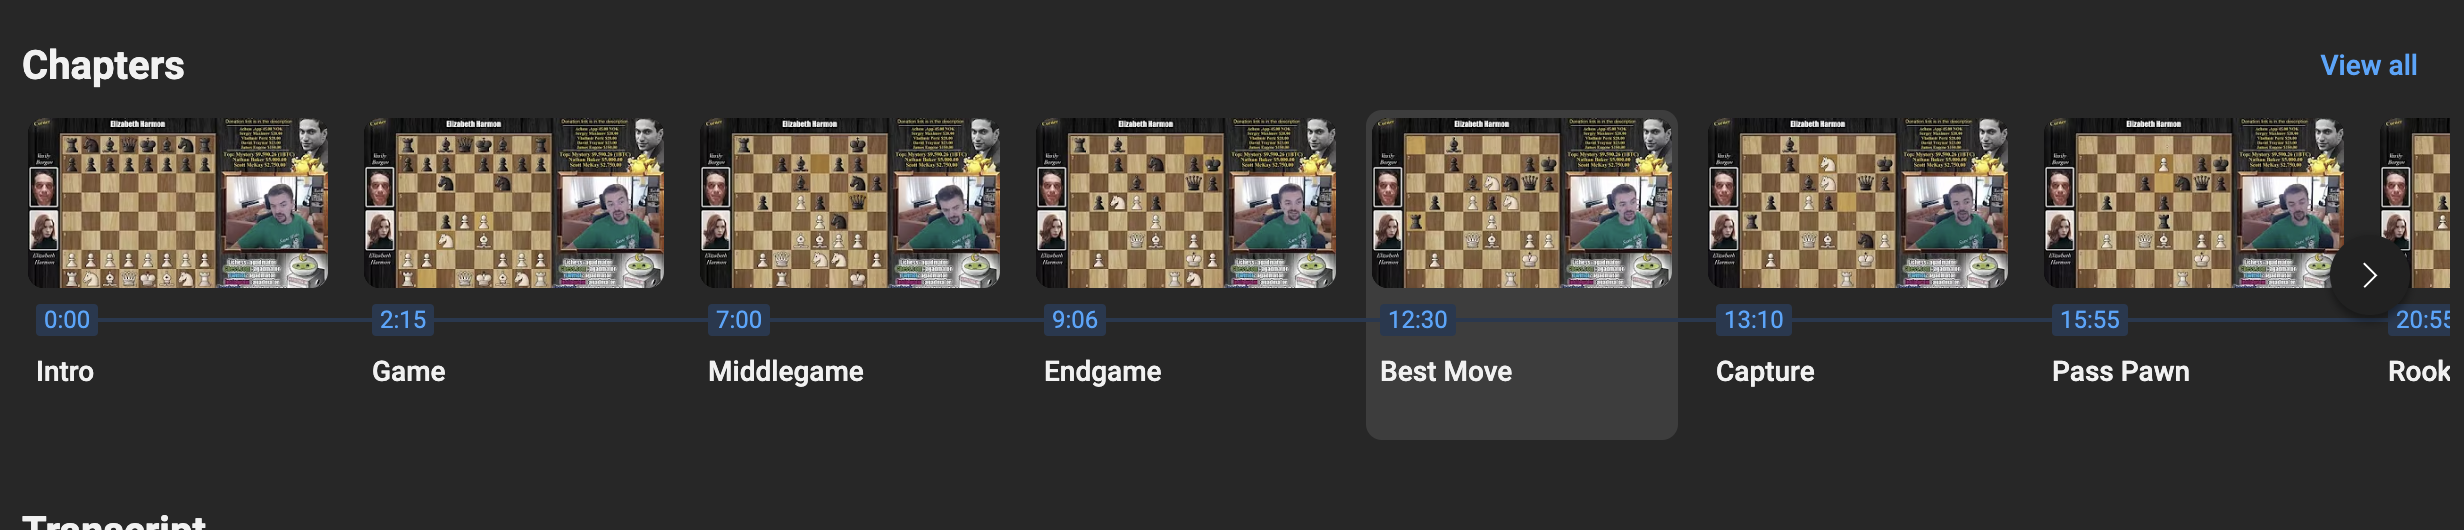
\includegraphics[width=\linewidth]{Screenshot 2025-01-22 at 5.18.04 PM.png}
    \caption{Game Commentary: Qualitative game segments annotated, with panel wise transcripts, compared with actual and GPT-4o}
    \label{fig:enter-label}
\end{figure}

\begin{figure}[!h]
     \centering
     \begin{subfigure}{0.45\textwidth}
         \centering
         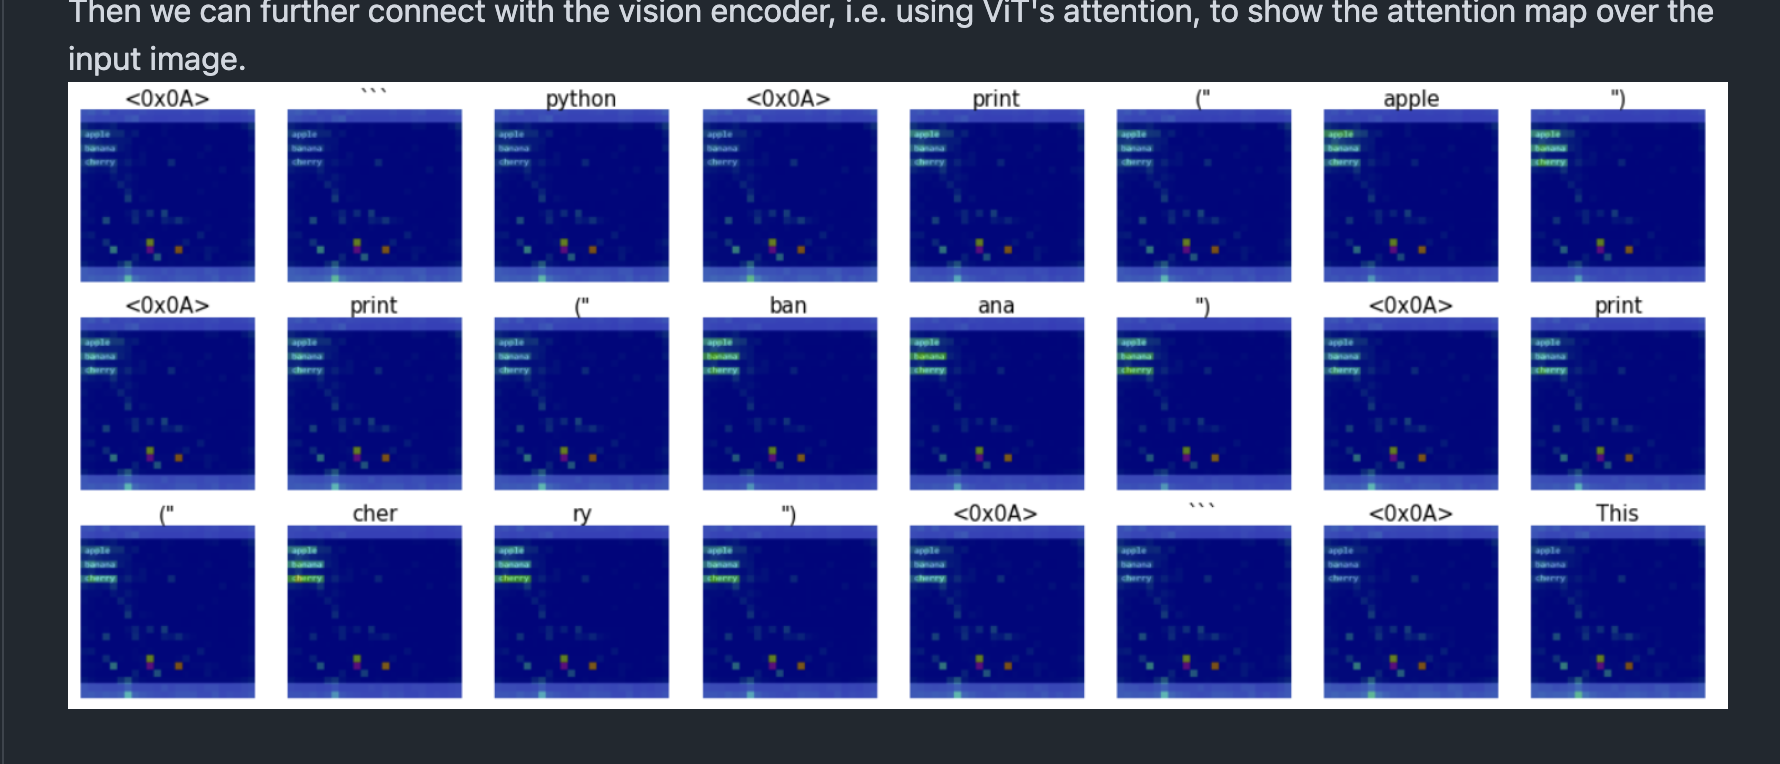
\includegraphics[width=\linewidth]{Screenshot 2025-01-22 at 5.46.55 PM.png}
         \label{fig:1a}
     \end{subfigure}
     \begin{subfigure}{0.45\textwidth}
         \centering
         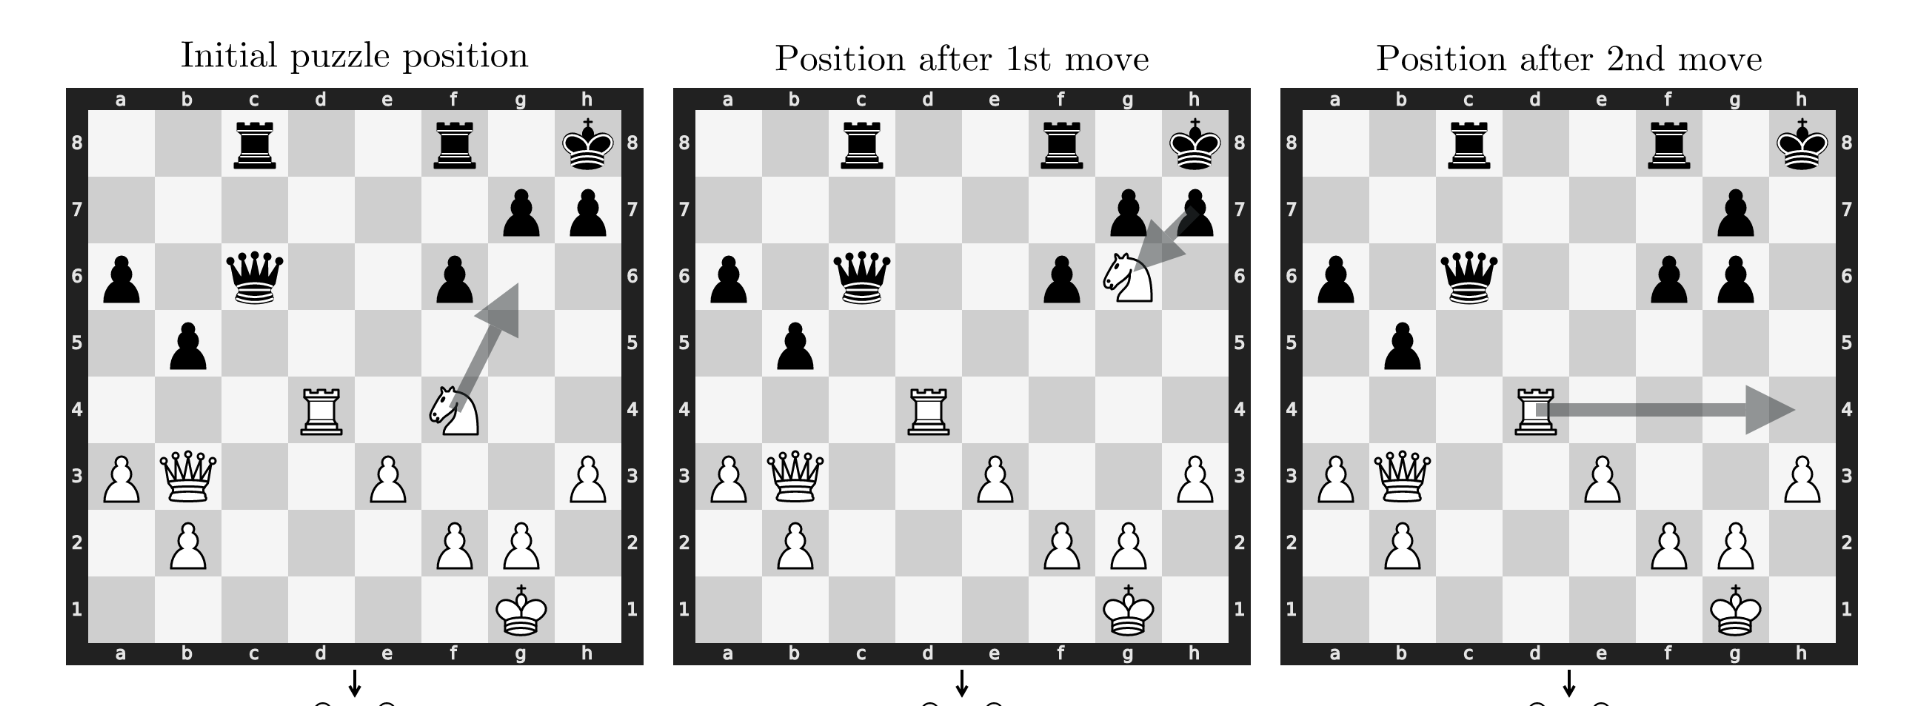
\includegraphics[width=\linewidth]{Screenshot 2025-01-22 at 5.50.06 PM.png}
         \label{fig:1b}
     \end{subfigure}
     \caption{Attention Visualization of board from decision tokens with different instruction on a position}
     \label{fig:1}
\end{figure}

\begin{figure}[!h]
    \centering
    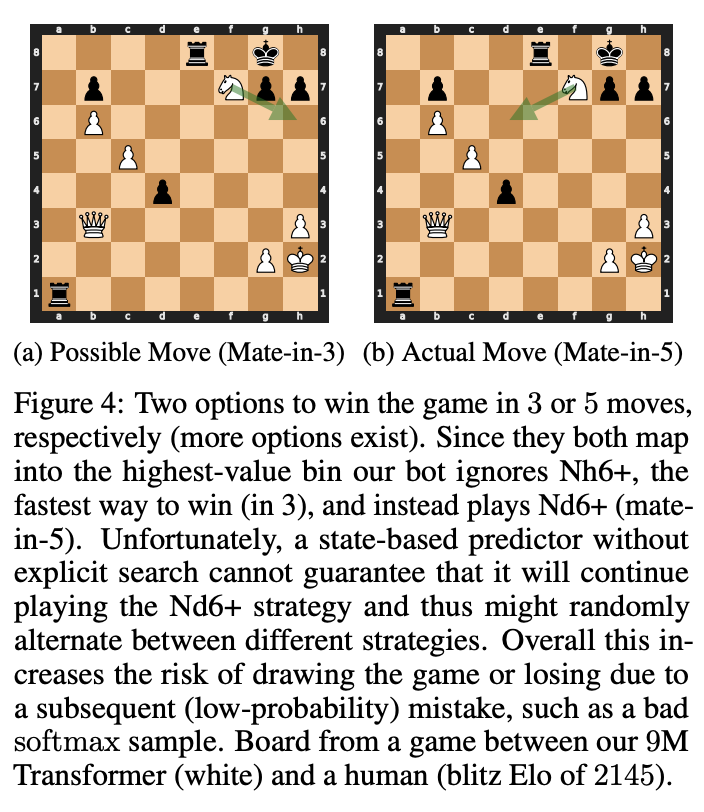
\includegraphics[width=\linewidth]{Screenshot 2025-01-22 at 5.39.44 PM.png}
    \caption{Move by move comparison on different BCL cases (Elo, DeltaElo, Time, Format)}
    \label{fig:enter-label}
\end{figure}

\subsubsection{Commentary}
We collect data of commentary on chess games from a famous Youtube channel called Agadmator aka Antonio Radić. On his channel, Radić reviews recent tournament games from top players, historical matches, and chess compositions. Almost all of Radić's videos follow the same format: a detailed analysis of one chess game. We extract paired commentary from the transcripts by aligning video clips with natural language transcripts based on timestamps.
\end{comment}

% \section{Introduction}
% \vspace{-2mm}

% % =============================================================================
% % PARAGRAPH 1: What is the problem?
% % =============================================================================

% Large language models excel at tasks solvable through next-token prediction over text, yet struggle in domains requiring multi-step reasoning over evolving states~\cite{valmeekam2022large,bachmann2024pitfalls}. Chess illustrates this gap concretely: despite extensive exposure to chess notation during pretraining, GPT-4 achieves approximately 1800 Elo---strong amateur level---while purpose-built engines exceed 3500 Elo~\cite{carlini2023chess,ruoss2024grandmaster}. Scaling alone does not close this gap; even with chess-specific fine-tuning, language models struggle at puzzles requiring multi-move lookahead~\cite{feng2024chessgpt}. The limitation appears structural: text-only models typically lack an internal representation of how actions change future states.

% In contrast, domain-specific agents trained through self-play or supervised learning achieve superhuman performance precisely because they learn such representations. A chess engine's internal state---which we term the \textit{latent state} $h_s = G_\psi(s)$---encodes not just a board position, but a probability distribution over legal moves, value estimates for future positions, and features capturing positional structure~\cite{silver2017mastering,schrittwieser2020mastering}. This representation enables the planning and lookahead that text-only LLMs lack. This contrast motivates our central question:

% \vspace{-2mm}
% \begin{quote}
%     {\fontsize{9.5pt}{11pt}\selectfont\textit{``What capabilities emerge when LLMs condition directly on the latent states of pretrained agents, rather than on their symbolic outputs?''}}
% \end{quote}
% \vspace{-1mm}

% % =============================================================================
% % PARAGRAPH 2: Why is it interesting and important?
% % =============================================================================

% This question matters because LLMs and domain-specific agents have complementary but non-overlapping strengths. LLMs excel at natural language understanding, instruction following, and leveraging broad world knowledge from pretraining. Domain-specific agents excel at precise action selection, value estimation, and implicit planning within their trained domains. If these capabilities could be combined effectively, the resulting system might perform tasks challenging for either component alone: explaining \textit{why} a position favors one side (requiring both positional understanding and language generation), adapting play style based on verbal instructions (requiring both language comprehension and policy modification), or predicting which positions humans find difficult (requiring both agent-level evaluation and human modeling).

% We formalize these target capabilities as two complementary paradigms. \textit{Generalized Decision Understanding} (GDU) encompasses tasks requiring reasoning about agent behavior---commentary generation, difficulty prediction, style identification. \textit{Generalized Decision Making} (GDM) encompasses tasks requiring action and policy adaptation---behavior cloning across skill levels, instruction-conditioned planning. Prior work has addressed these tasks individually with specialized models; our goal is a unified framework where both emerge from conditioning on latent states.

% % =============================================================================
% % PARAGRAPH 3: Why is it hard? (Why do naive approaches fail?)
% % =============================================================================

% The standard approach to combining LLMs with external agents is \textit{tool calling}: the LLM invokes an engine through a text interface and conditions on the returned output. While effective for language-native tools (calculators, code interpreters), this paradigm introduces an information bottleneck for agents whose reasoning occurs in continuous latent spaces. When an LLM queries a chess engine, even an enriched response---top-$k$ moves with evaluations, principal variation, win/draw/loss probabilities---remains a \textit{symbolic compression} of the agent's internal state. The latent representation $h_s$ encodes a full distribution over ${\sim}30$ legal moves, uncertainty quantification, and features capturing piece activity, king safety, and pawn structure. This information enables the agent's reasoning but does not transfer through the text interface.

% We emphasize that our critique is not that tool calling fails entirely, but that it imposes a ceiling on fine-grained tasks. A tool-calling LLM observes the \textit{outputs} of agent reasoning; a latent-conditioned LLM can access the \textit{substrate} of that reasoning. This distinction matters most for tasks requiring nuanced understanding: predicting how a 1600-Elo human would play (requiring the full policy distribution, not just the top move), generating commentary that captures positional subtlety (requiring evaluation features, not just scalar scores), or adapting strategy based on opponent weaknesses (requiring controllable policy modification, not just action selection).

% % =============================================================================
% % PARAGRAPH 4: Why hasn't it been solved before? (What's wrong with prior work?)
% % =============================================================================

% Prior work has pursued two main paradigms, each with limitations for our target tasks. The first, exemplified by ChessGPT~\cite{feng2024chessgpt}, fine-tunes LLMs on move sequences and natural language annotations. ChessGPT achieves reasonable playing strength and can generate chess-related text, but operates entirely in token space---it learns statistical patterns over notation rather than gaining access to structured agent representations. We show empirically (Section~\ref{sec:experiments}) that ChessGPT struggles with tasks requiring policy-level reasoning, such as predicting moves at specific Elo levels or adapting play to stated opponent weaknesses.

% The second paradigm, pioneered by vision-language models~\cite{liu2023visual,li2023blip}, projects encoder representations into the LLM's token space through learned adapters. This approach enables LLMs to reason over images and has inspired work connecting policies to language~\cite{brohan2023rt2,driess2023palme}. However, these projections are typically \textit{static}: the input is processed once and remains fixed throughout generation. In sequential decision domains, this assumption breaks---the LLM's action changes the environment state, which must be re-encoded by the agent for continued reasoning. Existing projection-based approaches lack a mechanism for this dynamic re-encoding, limiting their applicability to iterative planning.

% % =============================================================================
% % PARAGRAPH 5: What are the key components of my approach and results?
% % =============================================================================

% We propose \textbf{latent state internalization}: projecting the agent's latent representation directly into the LLM's token embedding space, with support for dynamic re-encoding during generation. A lightweight adapter $H_\phi: \mathbb{R}^d \rightarrow \mathbb{R}^{k \times e}$ maps the agent's latent state $h_s$ to $k$ tokens in the LLM's embedding space. These tokens are interleaved with language and action tokens during training and inference. Crucially, a special \texttt{<InvokeAgent>} token enables dynamic updates: when generated, the environment transitions based on the preceding action, the agent re-encodes the new state, and fresh latent tokens are appended. This closed loop supports iterative reasoning without external API calls.

% We instantiate this framework as \textbf{LLAMIA} (Large Language and Action Models with Internal Agents), combining Vicuna-7B/13B with the Lc0-BT4 chess engine (240M parameters). Training follows \textbf{SALT} (State, Action, Language Tokens): Stage 1 aligns the projection layer via state-to-description reconstruction; Stage 2 fine-tunes on interleaved sequences spanning gameplay, commentary, and instruction-following. We compare against ChessGPT-13B (fine-tuning baseline, same compute budget), GPT-4o with Stockfish tool access (tool-calling baseline, 5 queries per position), and Maia~\cite{mcilroy2020aligning} (specialized behavior cloning). Key findings:

% \begin{itemize}[leftmargin=*, topsep=2pt, itemsep=2pt]
%     \item \textbf{Data efficiency:} LLAMIA achieves policy alignment (Kendall's $\tau = 0.55 \pm 0.02$) with 50k pretraining games; ChessGPT-13B requires 200k games to match---a \textbf{4$\times$ data reduction} (Figure~\ref{fig:kt}, $n{=}5$ seeds, $p{<}0.01$ via paired $t$-test).
    
%     \item \textbf{Behavior cloning:} LLAMIA-13B achieves $55.0\% \pm 1.2\%$ move-matching accuracy on Elo-bucketed human games, vs.\ $48.2\%$ for Maia-best-of-9 and $41.3\%$ for GPT-4o with tool access (Table~\ref{tab:behavior}, $n{=}10$k positions).
    
%     \item \textbf{Conditional planning:} When instructed to exploit a stated weakness (``poor endgame play''), LLAMIA wins $62\% \pm 4\%$ vs.\ $45\%$ uninstructed---a \textbf{+17\% win rate} from language-based policy modification (Figure~\ref{fig:icp}, $n{=}200$ games).
    
%     \item \textbf{Commentary generation:} Human evaluators prefer LLAMIA's game-level commentary over GPT-4o with tool access $65\%$ vs.\ $35\%$ (Figure~\ref{fig:comm}, $n{=}100$ games, $p{<}0.01$ via binomial test).
% \end{itemize}

% We also demonstrate extensibility beyond chess: internalizing a reward model improves text-to-image preference prediction, and internalizing a persuasion classifier improves marketing analysis (Section~\ref{sec:extensions}). However, our core contribution is methodological---establishing latent internalization as a more efficient paradigm than tool calling for LLM-agent integration---with chess providing controlled experimental validation.

% % =============================================================================
% % SUMMARY OF CONTRIBUTIONS
% % =============================================================================

% \vspace{-1mm}
% \subsection{Summary of Contributions}
% \vspace{-1mm}

% \begin{enumerate}[leftmargin=*, labelsep=0.5em, topsep=2pt, itemsep=2pt]
%     \item \textbf{Latent State Internalization (Section~\ref{sec:method}):} A paradigm for LLM-agent integration where the agent's latent representation is projected into the LLM's token space, enabling conditioning on rich internal state rather than sparse symbolic outputs. We formalize the objective (Eq.~\ref{eq:intern}) and contrast with tool calling (Eq.~\ref{eq:tool}).
    
%     \item \textbf{SALT Training Framework (Section~\ref{sec:salt}):} A two-stage methodology---projector alignment followed by interleaved fine-tuning---achieving 4$\times$ data efficiency over language-only fine-tuning on policy alignment.
    
%     \item \textbf{Emergent GDU/GDM Capabilities (Section~\ref{sec:experiments}):} Empirical demonstration that latent internalization enables capabilities limited in tool-calling and fine-tuning baselines: controllable policy modification (+17\% win rate), accurate cross-Elo behavior cloning (55\% accuracy), and preferred game-level commentary (65\% preference).
    
%     \item \textbf{LLAMIA-Bench (Section~\ref{sec:benchmark}):} A benchmark for evaluating LLM-agent systems on generalized decision making and understanding, with tasks for conditional planning, behavior cloning, commentary generation, and state annotation.
% \end{enumerate}

% \vspace{-2mm}


% % 

\section{Results Synthesis and Paper Positioning}
\label{sec:results_synthesis}

% This section synthesizes experimental evidence to determine the optimal paper narrative and contribution ordering.

\subsection{Table-by-Table Key Insights}

\paragraph{Gameplay (Table~\ref{tab:gameplay-performance})}
\textbf{Primary Claim:} Latent internalization achieves 500$\times$ data efficiency over supervised transformers.
\textbf{Key Delta:} LLAMIA-13B (2279 Elo, 30M positions) matches Transformer-270M (2299 Elo, 15B positions) with 500$\times$ fewer training positions.
\textbf{Insight:} Pretrained agent knowledge transfers efficiently through projection; the LLM does not need to re-learn positional evaluation from scratch.
\textbf{Contribution Link:} Supports SALT framework as enabling efficient knowledge transfer.

\paragraph{Game-Level Commentary (Table~\ref{tab:game_commentary_annotation})}
\textbf{Primary Claim:} A 13B model with internalized agents outperforms 405B models with tool-calling on complex reasoning tasks.
\textbf{Key Delta:} LLAMIA-13B achieves G-eval 0.61 vs GPT-4o+Lc0 at 0.52 (+17.3\%); Highlight RMSE 5.09 vs 12.31 (+142\% improvement).
\textbf{Insight:} Tool-calling compresses agent state into sparse outputs; internalization preserves the full policy distribution needed for nuanced commentary.
\textbf{Contribution Link:} Directly supports dynamic projection over tool-calling paradigm.

\paragraph{Behavior Cloning (Table~\ref{tab:behavior_cloning})}
\textbf{Primary Claim:} One unified model replaces five task-specific experts while using 12$\times$ less data.
\textbf{Key Delta:} LLAMIA-13B (single model, 1M samples) achieves 0.52-0.55 accuracy across Elo buckets vs Maia (5 models, 12M samples each) at 0.46-0.55.
\textbf{Insight:} The LLM's language conditioning enables skill-level adaptation that specialized models achieve only through separate training.
\textbf{Contribution Link:} Supports unified GDU/GDM as emergent capability.

\paragraph{State Annotation (Table~\ref{tab:state_commentary_annotation})}
\textbf{Primary Claim:} Latent internalization enables counterfactual reasoning that tool-calling cannot support.
\textbf{Key Delta:} LLAMIA-13B achieves 38.13 BLEU-2 on Planning vs GPT-4o+Lc0 at 30.13 (+26.6\%).
\textbf{Insight:} Planning commentary requires reasoning about ``what would happen if...'' which demands continuous access to agent representations, not discrete API calls.
\textbf{Contribution Link:} Strongest evidence for dynamic re-encoding necessity.

\paragraph{Puzzle Understanding (Table~\ref{tab:puzzle_understanding})}
\textbf{Primary Claim:} Internalized representations capture human-aligned difficulty perception.
\textbf{Key Delta:} LLAMIA-13B achieves $\rho=0.70$ on difficulty prediction vs GPT-4o+Lc0 at $\rho=0.53$ (+32\%).
\textbf{Insight:} The agent's latent state encodes features correlated with human difficulty (piece coordination, pattern recognition) that don't transfer through symbolic outputs.
\textbf{Contribution Link:} Supports latent states capturing richer information than tool outputs.

\paragraph{Conditional Planning (Table~\ref{tab:instruct_conditioned_planning})}
\textbf{Primary Claim:} Language-conditioned policy modification requires iterative state updates.
\textbf{Key Delta:} LLAMIA-13B achieves 17\% win-rate improvement vs LLaMA-3.1 405B+Lc0 at 10\% (+70\% relative improvement).
\textbf{Insight:} Exploiting opponent weaknesses requires steering play toward specific positions over multiple moves—a task requiring the \texttt{<InvokeAgent>} mechanism for ongoing state evaluation.
\textbf{Contribution Link:} Strongest validation of dynamic re-encoding for multi-step planning.

\subsection{Ablation Synthesis: What Drives Performance?}

\paragraph{Most Critical: Dynamic Re-Encoding (InvokeAgent)}
The InvokeAgent ablation (Table~\ref{tab:invoke_ablation}) reveals the starkest asymmetry:
\begin{itemize}[leftmargin=*, itemsep=1pt]
    \item \textbf{Single-step tasks:} Gameplay (-1.3\%), BC (-3.8\%) — minimal degradation
    \item \textbf{Multi-step tasks:} Planning (-64.3\%), Commentary (-22.4\%) — severe degradation
\end{itemize}
\textbf{Causal Chain:} Multi-step tasks (conditional planning, game commentary) require reasoning over \textit{evolving} states. Static projection—like tool-calling—provides a snapshot; InvokeAgent enables a closed-loop where the LLM's actions update the environment and fresh latent states are re-encoded. This is the \textbf{key differentiator} over all baselines.

\paragraph{Supporting: Two-Stage Training}
Stage 1 alone achieves strong gameplay (2198 Elo) but poor language tasks (Commentary 0.31). Stage 2 alone shows instability. Full SALT combines both benefits.
\textbf{Insight:} Stage 1 provides stable projector initialization from abundant synthetic data; Stage 2 enables task-specific adaptation. Neither alone is sufficient.

\paragraph{Scaling: Agent Quality}
Performance scales linearly with agent Elo (T72→BT4 gives +258 Elo, +7\% planning win-rate).
\textbf{Insight:} LLAMIA inherits and amplifies agent capabilities—stronger agents yield proportionally better LLM performance.

\subsection{Story Recommendation}

We evaluate four candidate narratives against the evidence:

\begin{enumerate}[label=\Alph*., leftmargin=*]
    \item \textbf{SALT-first:} ``Unified modeling of States, Actions, Language enables emergent capabilities''
    \item \textbf{Dynamic Projector-first:} ``InvokeAgent enables iterative reasoning over evolving states''
    \item \textbf{Data Efficiency-first:} ``Latent internalization achieves 50-500$\times$ data efficiency''
    \item \textbf{Unified Model-first:} ``One model replaces multiple task-specific experts''
\end{enumerate}

\paragraph{Recommendation: B (Dynamic Projector) as primary, supported by A (SALT)}

\textbf{Rationale:}
\begin{enumerate}[leftmargin=*, itemsep=2pt]
    \item \textbf{Falsifiability:} The InvokeAgent ablation provides direct causal evidence. Reviewers can verify: ``remove InvokeAgent → planning collapses''.
    \item \textbf{Differentiation:} Dynamic re-encoding is what separates LLAMIA from (a) tool-calling (static API outputs), (b) VLMs (static image encoding), and (c) ChessGPT (no agent at all).
    \item \textbf{Generalizability:} The mechanism—LLM generates actions, invokes agent to re-encode updated state—applies to robotics, games, and any sequential decision domain.
    \item \textbf{Memorability:} ``The LLM operates state evolution as a tool call'' is a crisp, memorable framing.
\end{enumerate}

SALT is the \textit{enabling framework} that makes dynamic re-encoding possible; data efficiency and unified capabilities are \textit{consequences}. The story should be: \textbf{``Dynamic re-encoding enables multi-step reasoning (B), implemented via SALT (A), achieving 500$\times$ data efficiency (C) and unified capabilities (D).''}

\subsection{Contribution Ordering}

Based on the synthesis above, we recommend the following ordering:

\begin{enumerate}[leftmargin=*, itemsep=4pt]
    \item \textbf{PRIMARY: Latent State Internalization with Dynamic Re-Encoding}
    
    \textit{``A paradigm for LLM-agent integration where the agent's latent representation is projected into the LLM's token space, with support for dynamic re-encoding during generation via the \texttt{<InvokeAgent>} mechanism.''}
    
    \textbf{Justification:} This is the core methodological innovation. Without InvokeAgent, planning drops 64\%; without projection, the entire approach collapses. This component has the highest Novelty $\times$ Impact.
    
    \item \textbf{SECONDARY: SALT Training Framework}
    
    \textit{``A two-stage training methodology—projector alignment followed by interleaved fine-tuning on State, Action, and Language tokens—achieving 4$\times$ data efficiency over language-only fine-tuning.''}
    
    \textbf{Justification:} SALT is the architectural scaffold that makes Contribution 1 possible. The two-stage design (Table~\ref{tab:stage_ablation}) is necessary for stable training. This provides the ``how'' to Contribution 1's ``what''.
    
    \item \textbf{TERTIARY: Emergent GDU/GDM Capabilities}
    
    \textit{``Empirical demonstration that latent internalization enables capabilities limited in baselines: controllable policy modification (+17\% win-rate), cross-Elo behavior cloning (55\% accuracy), and preferred commentary (G-eval 0.61).''}
    
    \textbf{Justification:} These are the consequences that validate Contributions 1 and 2. Strong empirically but derivative conceptually.
    
    \item \textbf{QUATERNARY: LLAMIA-Bench}
    
    \textit{``A benchmark for evaluating LLM-agent systems on generalized decision making and understanding, with tasks for conditional planning, behavior cloning, commentary, and state annotation.''}
    
    \textbf{Justification:} Valuable for reproducibility and future work, but secondary to the methodological contributions.
\end{enumerate}

\subsection{Reviewer-Ready Pitch}

The paper's core claims, in descending order of importance:

\begin{enumerate}[leftmargin=*, itemsep=3pt]
    \item \textbf{Dynamic projection enables iterative reasoning over evolving states}, unlocking multi-step planning that tool-calling cannot support. Evidence: 17\% planning win-rate improvement; 64.3\% drop when InvokeAgent is removed; Commentary G-eval 0.61 vs 0.52 for GPT-4o+Lc0.
    
    \item \textbf{Latent internalization achieves 500$\times$ data efficiency} by leveraging pretrained agent knowledge. Evidence: 30M positions vs 15B for comparable Elo; 1 model vs 5-model ensemble for behavior cloning; 1M samples vs 12M for Maia-level accuracy.
    
    \item \textbf{Unified modeling enables a 13B model to outperform 30$\times$ larger LLMs with tool-calling} on reasoning-intensive tasks. Evidence: +26.6\% on Planning BLEU-2 vs GPT-4o+Lc0; +17.3\% on G-eval vs GPT-4o+Lc0; +32\% on difficulty prediction $\rho$.
\end{enumerate}

\subsection{The Paper Story}

\textbf{One-line pitch:} LLAMIA internalizes pretrained agents into LLMs via dynamic latent projection, enabling iterative reasoning over evolving states that tool-calling cannot support.

\textbf{Expanded narrative:}
Large language models excel at language but struggle with multi-step reasoning over structured states. The dominant paradigm—tool-calling—compresses rich agent representations into sparse symbolic outputs, creating an information bottleneck. We propose \textit{latent state internalization}: projecting the agent's continuous representation directly into the LLM's token space, with a novel \texttt{<InvokeAgent>} mechanism for dynamic re-encoding during generation. This closed loop enables the LLM to reason over evolving states—critical for planning, commentary, and policy adaptation.

We instantiate this as LLAMIA, combining Vicuna with the Lc0 chess engine. Key findings:
\begin{itemize}[leftmargin=*, itemsep=1pt]
    \item Removing InvokeAgent causes 64\% degradation on planning but only 1\% on single-step tasks, confirming that dynamic re-encoding is \textit{specifically} critical for multi-step reasoning.
    \item A 13B LLAMIA outperforms 405B models with tool-calling on commentary (G-eval 0.61 vs 0.52) and planning (+7\% win-rate), demonstrating that latent internalization overcomes the tool-calling bottleneck.
    \item Extensions to vision (ImageReward internalization) and persuasion (Chronos internalization) show the approach generalizes beyond chess.
\end{itemize}

The contribution is not ``better chess AI'' but a \textbf{paradigm for LLM-agent integration} that applies wherever iterative reasoning over structured states is needed: robotics, autonomous driving, game AI, and beyond.

